\chapter{Results}
\section{Segmentation}
The proposed measures mentioned in Section~\ref{sec:carotid} significantly improved carotid segmentation by excluding lesions and unwanted venous.
As apparent by Figure~\ref{fig:seg_compare}, we can see the importance of the cuboid mask.
Since the segmentation does not have a ground truth to be compared to, visual inspection of the segmentation showed promising results and lesions and venous were rarely selected by the algorithm.
% However, the algorithm would 
% Although the measures in Section~\ref{sec:carotid} significantly improved carotid segmentation by excluding lesions and venous tissues, there is still room for improvement.
However, the algorithm became overly conservative.
In some cases, even though no non-carotid tissues were selected, parts of the carotid structure were excluded.
In other cases, the cuboid mask registration either failed entirely or was insufficiently accurate, resulting in the exclusion of parts of the carotid structure.

\begin{figure}[h]
	\centering
	\begin{subfigure}{0.45\textwidth}
		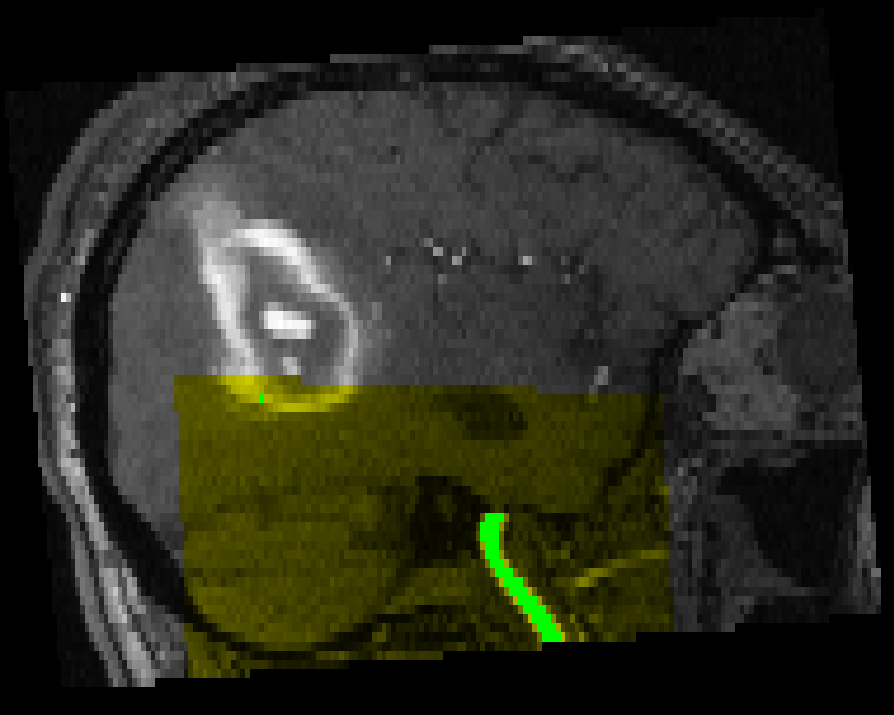
\includegraphics[width=\textwidth]{figures/molgu07704_bbox.png}
		\caption{}
		\label{subfig:seg_bbox}
	\end{subfigure}
	\begin{subfigure}{0.45\textwidth}
		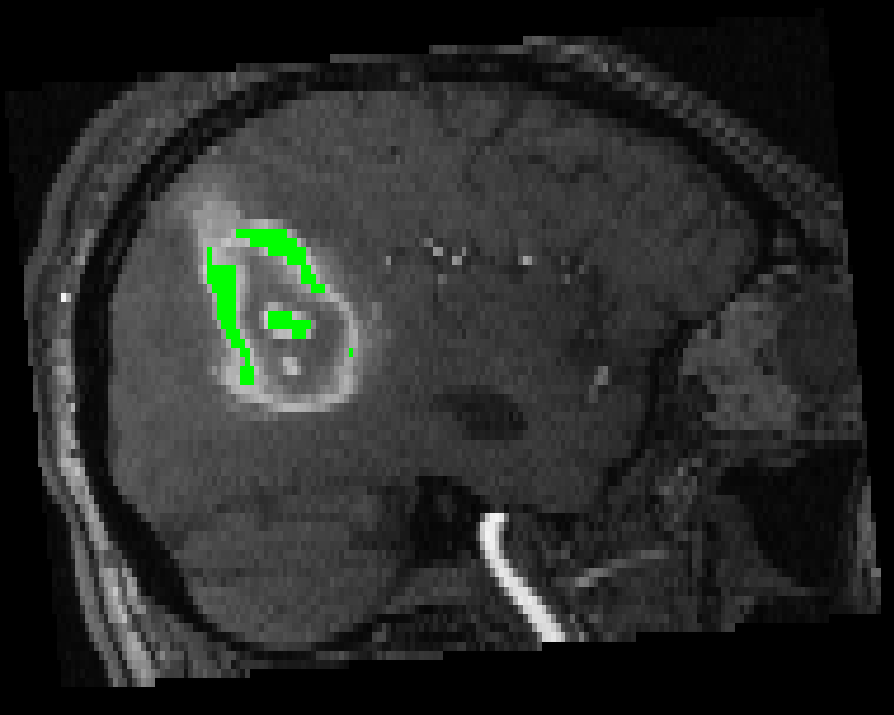
\includegraphics[width=\textwidth]{figures/molgu07704_nobbox.png}
		\caption{}
		\label{subfig:seg_nobbox}
	\end{subfigure}
	\caption{Comparison of carotid segmentation (green) with (a) and without (b) a cuboid mask (yellow). In the absence of the cuboid mask, the segmentation algorithm fails to capture the carotid and instead incorrectly identifies the brain lesion}
	\label{fig:seg_compare}
\end{figure}

\section{IDIF}
IDIF estimation was performed using both the Bayesian GTM (BGTM) and the GTM PVC method. The average mean absolute error (MAE) of the cAUC across the dataset was 14,202 for BGTM and 33,764 for GTM.

ROI‐based quantification was carried out using both IDIFs, with BGTM yielding significantly better performance. BGTM and GTM methods acheived an Average \(\mrglu\) MAPE of 14.1\% and 33\%, and an AVERAGE \(\mrglu\) MAE of 1.42 and 3.5, respectively.
Additionally, \(R^2\) MAE and \(S\) MAE were 0.004 and 0.14 for BGTM, and 0.030 and 0.304 for GTM, respectively.

As seen in Figure~\ref{fig:corr_mat}, there is high correlation between the MAE cUAC curve error and the mentioned quantification errors. \pdfcomment{ok what eles? thats it?}

\begin{table}
	\centering
	\begin{tabular}{l|cc|cc}
		\toprule
		\multirow{2}{*}{\textbf{Metric}} & \multicolumn{2}{c|}{\textbf{BGTM}} & \multicolumn{2}{c}{\textbf{GTM}}                        \\
		\cmidrule(lr){2-3} \cmidrule(lr){4-5}
		                                 & \(\mu\)                            & \(\sigma\)                       & \(\mu\) & \(\sigma\) \\
		\midrule
		cAUC MAE                         & 14,202                             & 9,190                            & 33,764  & 21,212     \\
		\(\textrm{MR}_{glu}\) MAPE (\%)  & \textbf{14.1}                      & \textbf{10.1}                    & 33.0    & 31.5       \\
		\(\textrm{MR}_{glu}\) MAE        & 1.42                               & 1.07                             & 3.50    & 3.38       \\
		\(R^2\) MAE                      & 0.004                              & 0.006                            & 0.030   & 0.132      \\
		Slope MAE                        & 0.14                               & 0.109                            & 0.304   & 0.230      \\
		\bottomrule
	\end{tabular}
	\caption{Summary of performance metrics for BGTM and GTM methods.}
	\label{tab:metrics}
\end{table}

\begin{figure}
	\centering
	\begin{subfigure}{\textwidth}
		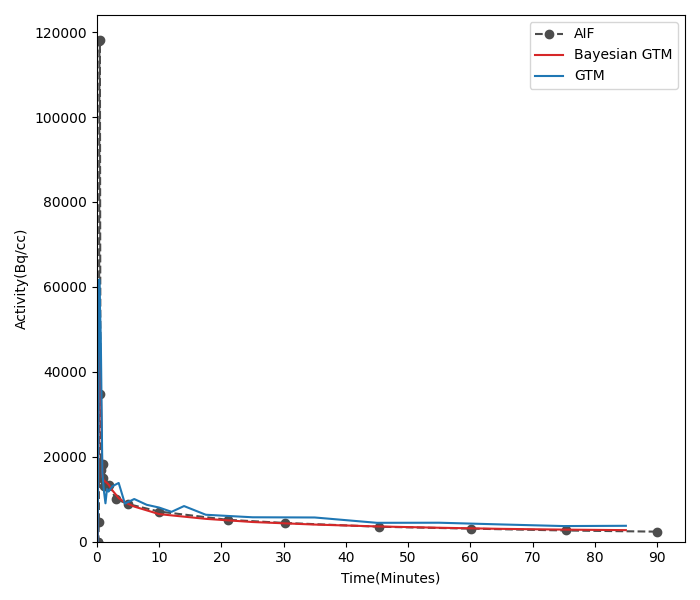
\includegraphics[width=\textwidth]{figures/RD11934_1_if_comparison.png}
		% \caption{Input function comparison}
		\label{subfig:if_compare}
	\end{subfigure}
	\begin{subfigure}{\textwidth}
		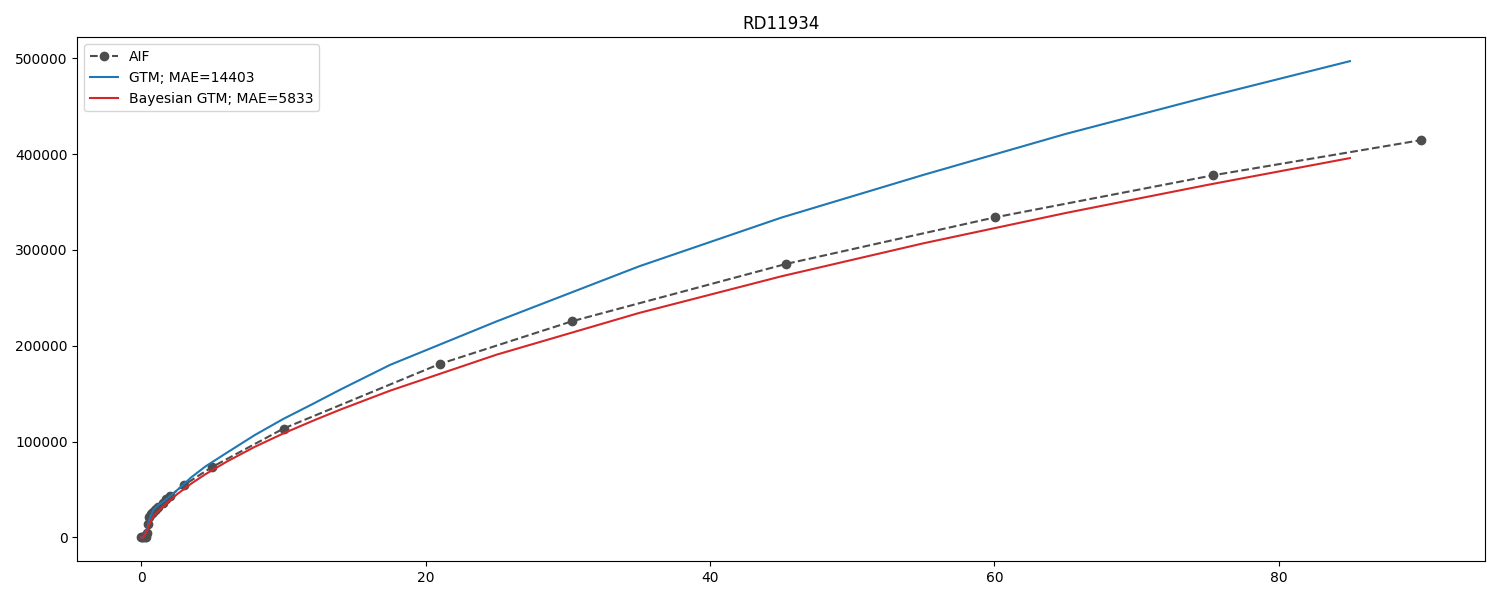
\includegraphics[width=\textwidth]{figures/RD11934_1_trap.png}
		% \caption{Cumulative AUC of IFs}
		\label{subfig:trap_compare}
	\end{subfigure}
	\label{fig:ifs}
	\caption{Comparison of the IFs (Top) and Cumulative AUC curves (Bottom) for a specific subject}
\end{figure}




\begin{figure}
	\centering
	\begin{subfigure}[b]{0.45\textwidth}
		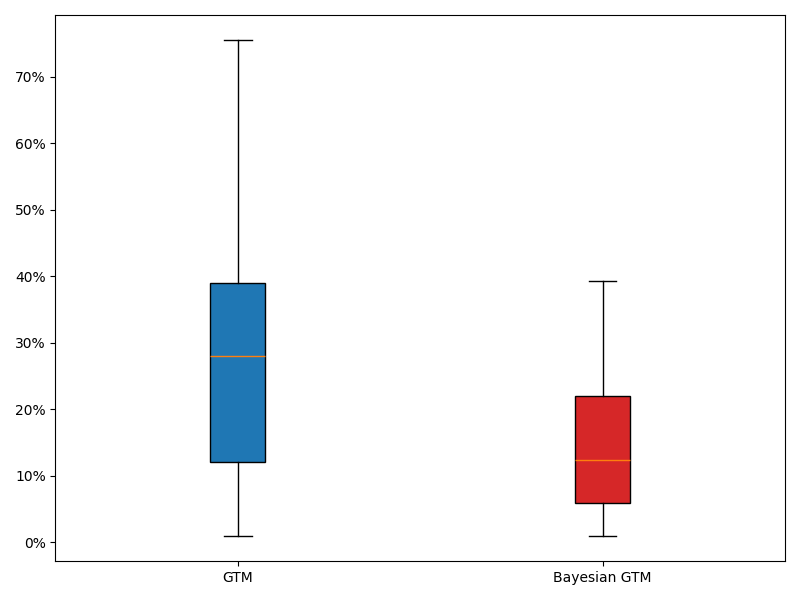
\includegraphics[width=\textwidth]{figures/quantification_mape_fitk3_boxplot.png}
		\caption{\(\mrglu\) MAPE Boxplot}
		\label{subfig:fitk3_mape}
	\end{subfigure}
	\begin{subfigure}[b]{0.45\textwidth}
		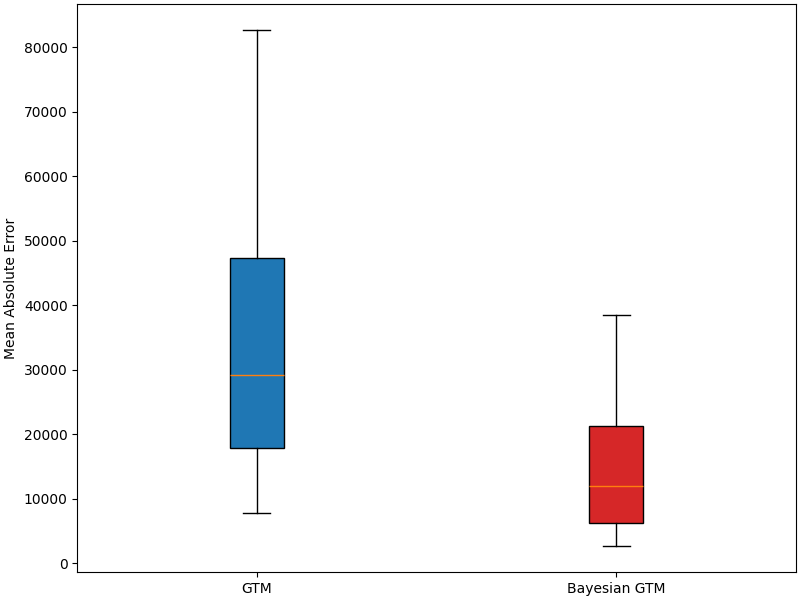
\includegraphics[width=\textwidth]{figures/curve_errors_boxplots.png}
		\caption{cAUC MAE Boxplot}
		\label{subfig:curve_errors_boxplot}
	\end{subfigure}
	\label{fig:boxplots}
	\caption{Boxplot of curve and quantification errors}
\end{figure}

\begin{figure}
	\centering
	\begin{subfigure}{0.45\textwidth}
		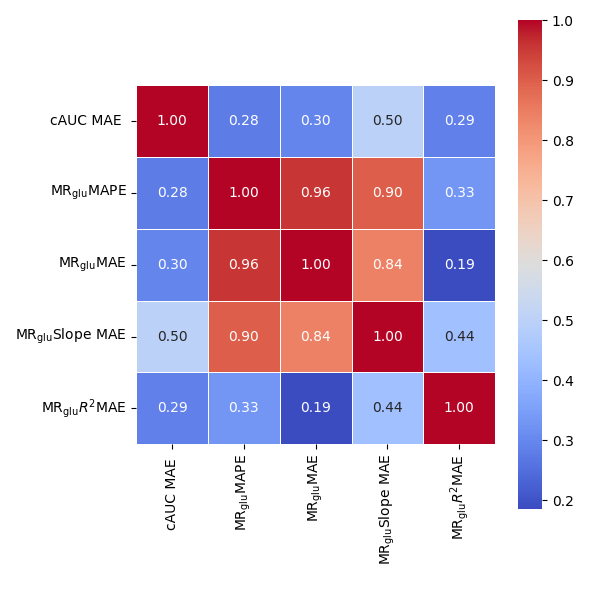
\includegraphics[width=\textwidth]{figures/corr_gtm.png}
		\caption{GTM}
		\label{subfig:corr_gtm}
	\end{subfigure}
	\begin{subfigure}{0.45\textwidth}
		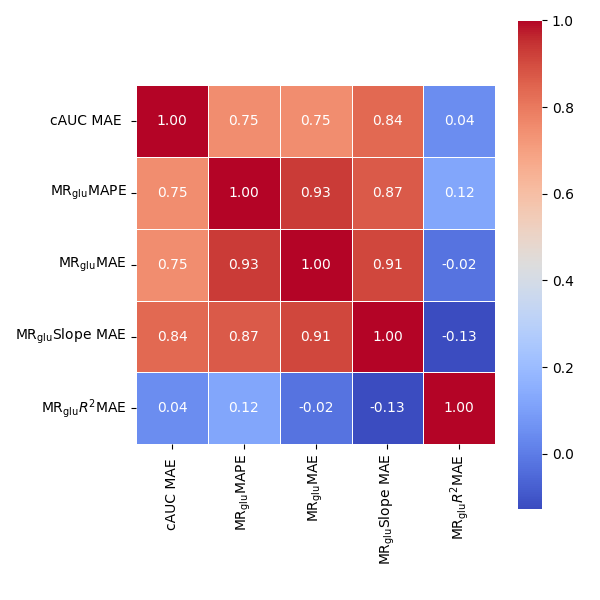
\includegraphics[width=\textwidth]{figures/corr_bgtm.png}
		\caption{Bayesian GTM}
		\label{subfig:corr_bgtm}
	\end{subfigure}
	\label{fig:corr_mat}
	\caption{Correlation matrix of different metrics for Bayesian GTM and GTM methods}
\end{figure}

% \section{IDIF}



